\documentclass[12pt]{article}

\usepackage{geometry}
\usepackage{amsmath, amsthm, amssymb}
\usepackage{graphicx}
\usepackage{tikz}
\usepackage{tkz-berge}
\usepackage{tkz-graph}
\usepackage{booktabs} % See the package documentation for guidelines on formal tables: https://ctan.org/pkg/booktabs
\usepackage{verbatim} % Used to typeset, for example, code snippets or pseudo-code for algorithms.
\usepackage{dsfont} % Extra fontset for helpful mathematics symbols, e.g. \mathds{1}
\usepackage{etoolbox} % Used to allow boolean variables for use in the title page
\usepackage{import}
\usepackage{lipsum}
\usepackage{subcaption}
\usepackage{float}
\usepackage{enumitem}
\usepackage{tabularx}
\usepackage{array}
\usepackage{pdfpages}
\usepackage{mathtools}
\usepackage{hyperref}
\usepackage{mathbbol}
\usepackage{caption}

\newcolumntype{C}[1]{>{\centering\arraybackslash}m{#1}}
\newcommand{\R}{\mathbb{R}}
\newcommand{\Q}{\mathbb{Q}}
\newcommand{\C}{\mathbb{C}}
\newcommand{\N}{\mathbb{N}}
\newcommand{\Z}{\mathbb{Z}}
\newcommand{\T}{\mathbb{T}}
\newcommand{\cA}{\mathcal{A}}
\newcommand{\cB}{\mathcal{B}}
\newcommand{\cD}{\mathcal{D}}
\newcommand{\cP}{\mathcal{P}}
\newcommand{\cM}{\mathcal{M}}
\newcommand{\abs}[1]{\left\lvert #1 \right\rvert}
\newcommand{\norm}[1]{\left\lVert #1 \right\rVert}
\newcommand{\set}[2]{\left\{#1 \ : \ #2\right\}}
\newcommand{\conv}[1]{\underset{#1}\longrightarrow}
\newcommand{\Mod}[1]{\ (\mathrm{mod}\ #1)}
\newcommand{\Supp}[0]{\ \mathrm{Supp}\ }
\DeclarePairedDelimiter\ceil{\lceil}{\rceil}
\DeclarePairedDelimiter\floor{\lfloor}{\rfloor}
\DeclareMathOperator{\lcm}{lcm}

\newcommand{\Cross}{\mathbin{\tikz [x=1.4ex,y=1.4ex,line width=.2ex] \draw (0,0) -- (1,1) (0,1) -- (1,0);}}

\newcommand\restr[2]{{% we make the whole thing an ordinary symbol
		\left.\kern-\nulldelimiterspace % automatically resize the bar with \right
		#1 % the function
		\vphantom{\big|} % pretend it's a little taller at normal size
		\right|_{#2} % this is the delimiter
}}
% Custom math operators (analogous to \lim, \sup, etc).
\DeclareMathOperator{\id}{id}
\DeclareMathOperator{\od}{od}
\DeclareMathOperator{\subspan}{span}
\DeclareMathOperator{\sgn}{sgn}
\DeclareMathOperator{\diam}{diam}
\DeclareMathOperator{\rad}{rad}
%\DeclareMathOperator{\span}{span}

\newtheorem{thm}{Theorem}[section] % Numbering is impacted by [chapter]; could do [section] or [subsection] also.
\newtheorem{lem}{Lemma} % The [thm] argument says to number Lemma in sequence with Theorem.
\newtheorem{prop}[thm]{Proposition}
\newtheorem{cor}[thm]{Corollary}
\newtheorem{conj}[thm]{Conjecture}
\newtheorem{question}{Question}
% These environments are unnumbered and will not count toward the numbering.
%\newtheorem*{question}{Question}
\newtheorem*{answer}{Answer}
\newtheorem*{conjecture}{Conjecture}
\newtheorem*{claim}{Claim}
% These environments are definitions; they have a different style (bold label, standard font).
\theoremstyle{definition}
\newtheorem{defn}[thm]{Definition} % These definitions are also numbered in sequence with Theorem.
\newtheorem{eg}{Example}
\newtheorem{rem}[thm]{Remark}
\newtheorem{obs}{Observation}

\title{ \vspace{-3cm} Distance Multiplicities and Triangle Bases of the Cycle Space}
\author{Tao Gaede}

\begin{document}
	\maketitle

\section{Summary}

This document summarizes a connection between graph distance multiplicities and cycle spaces.  We present some basic lower and upper bounds that are immediately implied from this connection, and also explore the possibility of finding a formula for distance multiplicities.  Using an example of a tree, we present and explore some structural connections to distance multiplicities, specifically, algebraic and combinatorial (special sets of triples).  We conclude with some general observations and an initial set of questions.

\section{Preliminary Notions}

Throughout this discussion, we assume that $G$ is a connected graph with no induced cycles of length at least $5$.  We denote $G^k$ as the $k$-th power of $G$, which has vertex set $V(G)$ and $u,v \in V(G)$ are adjacent if and only if $d(u,v) \leq k$.  Our restriction that $G$ has no induced cycle of length at least $5$ means that all of its powers are chordal, which is necessary for our discussion insofar as it relates to triangles.  For each $k \in \{1, 2, \ldots, \diam(G)\}$, we use $m(k)$ to denote the multiplicity of distance $k$ in $G$.  Notice that $m(k) = |E(G^k)| - |E(G^{k-1})|$.  So, to find $m(k)$ it is sufficient to bound the size of powers of $G$.

Recall that the cycle space of a graph $G$, denoted $\mathcal{C}(G)$, is the subspace of the edge space $\mathbb{F}_2^{|E(G)|} \subseteq \mathbb{F}_2^{n \choose 2}$ that contains all eulerian subgraphs of $G$.  Let $c$ be the number of components of $G$.  The dimension of the cycle space has a formula:
$$\dim \mathcal{C}(G) =  |E(G)| - n + c.$$

\section{Enumeration Discussion: Bounding and Approximating Multiplicities}
The cycle space has a basis of special cycles called \emph{fundamental cycles}, which are characterized as follows: let $T$ be a spanning tree of $G$; then for each edge $uv \in E(G) \setminus E(T)$, the unique cycle of $T + uv$ is a fundamental cycle.  Since the base field is $\mathbb{F}_2$, addition of two subgraphs is the symmetric difference of their edges.  It follows that all fundamental cycles can be generated by the induced cycles of $G$.  Note that if $G$ is chordal, then all induced cycles are triangles.  Since $G$ is connected with no induced cycles of length at least $5$, its powers are chordal, so their cycle spaces are spanned by triangles.  However, the set of all triangles do not necessarily form a basis.

Let $A(G)$ be the adjacency matrix of $G$.  Then based on the above, we immediately have an upper bound on $\dim\mathcal{C}(G^k)$ as the number of triangles in $G^k$:  
$$\dim\mathcal{C}(G^k) \leq t_k,$$
where $t_k := \tfrac{Tr(A^3(G^k))}{6}$.  For a lower bound, we use a result of Hong Yuan\footnote{The paper is \textit{A Bound on the Spectral Radius of Graphs} (1988).  There are better more recent bounds if needed.  The most recent one I saw was from 2019, but Hong's proof and bound are relatively simple} on an upper bound for the spectral radius $\rho_k$ of $A(G^k)$ in terms of size and order:
$$\rho \leq \sqrt{2|E| - n + 1}.$$  
Rearranging, we can lower bound $\dim\mathcal{C}(G^k)$ as follows:
$$\frac{\rho_k^2 - (n-1)}{2} \leq \dim \mathcal{C}(G^k).$$

Notice that $m(k) = \dim \mathcal{C}(G^k) - \dim \mathcal{C}(G^{k-1})$, because the $(n-1)$ from each cancel.  So, putting the above two bounds together gives us bounds on $m(k)$:
$$\tfrac{1}{2}(\rho_k^2 - n+1)- t_{k-1} \leq m(k) \leq t_k - \tfrac{1}{2}(\rho_{k-1}^2 - n+1).$$

We call a basis for $\mathcal{C}(G^k)$ involving only triangles a \emph{$k$-triangle basis for $G$}.  Since $k$-triangle bases are obviously a subset of all triangles, it is probably reasonable to expect that $t_k$ can be scaled using an algebraic parameter related to $A(G^k)$ so that the result counts the number of independent triangles in a basis for $\mathcal{C}(G^k)$.  

Computer experimentation on small order trees suggests that one can get quite close to $\dim \mathcal{C}(G^k)$, for $k \in [3,\diam(G)]$, by simply dividing by $\tfrac{\rho_k}{2}$:
$$\dim \mathcal{C}(G^k) \sim \frac{2t_k}{\rho_k} + \Theta(n).$$

So, it appears that a formula for $m(k)$ in terms of $A(G^k)$ could be within reach.  I don't know why this approximation is so close -- somehow dividing by $\rho$ removes a lot of (oriented) dependent triangles.  This estimate is really good for $n \leq 13$ or so, in that it approximates $m(k)$ within an error of about $2$ or $3$, however the error increases with the order, and the estimate seems to become a lower bound for $k \in [3,\diam(G)]$, so the estimate misses some independent triangles.  

Again, this experimentation was only done on trees, so maybe tree structure is coming into play here to make the estimate closer than in general.  However, I would expect this estimate to work equally well for any $G$ with $G^k$ chordal.  Not sure though.

\section{Structural Discussion: Related Matrices and Triple Systems}



\begin{eg}
Below is an example of a tree of order $7$ and diameter $4$ and its associated $k$ powers and triangle bases.  Note that these bases form a nested sequence.  The triangle bases for these graphs are as follows:
\begin{align*}
	\mathcal{T}(T) &=  \emptyset	\\
	\mathcal{T}(T^2) &= \{160, 460, 450, 140, 130, 230, 120\}	\\
	\mathcal{T}(T^3) &= \{160, 460, 450, 140, 130, 230, 120, 260, 360, 560, 150, 240, 340\}	\\
	\mathcal{T}(T^4) &= \{160, 460, 450, 140, 130, 230, 120, 260, 360, 560, 150, 240, 340, 350, 250\}
\end{align*}
Observe that the differences in dimensions of consecutive cycle spaces are the multiplicities of the distances $k \in \{2, 3, 4\}$ of $T$.  That is, we have $m(2) = 7$, $m(3) = 6$, $m(4) = 2$.  Since $m(1) = |E(T)| = n-1 = 6$, and there are ${n \choose 2} = 21$ distances, all are accounted for.  Below are the graph powers of $T$.
		\begin{figure}[htbp]
		\begin{subfigure}[s]{0.3\textwidth}
			\begin{center}
			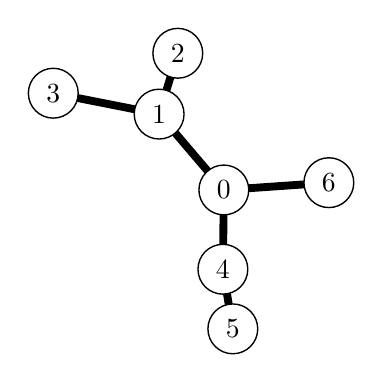
\begin{tikzpicture}[scale=0.70]
				\definecolor{cv0}{rgb}{0.0,0.0,0.0}
				\definecolor{cfv0}{rgb}{1.0,1.0,1.0}
				\definecolor{clv0}{rgb}{0.0,0.0,0.0}
				\definecolor{cv1}{rgb}{0.0,0.0,0.0}
				\definecolor{cfv1}{rgb}{1.0,1.0,1.0}
				\definecolor{clv1}{rgb}{0.0,0.0,0.0}
				\definecolor{cv2}{rgb}{0.0,0.0,0.0}
				\definecolor{cfv2}{rgb}{1.0,1.0,1.0}
				\definecolor{clv2}{rgb}{0.0,0.0,0.0}
				\definecolor{cv3}{rgb}{0.0,0.0,0.0}
				\definecolor{cfv3}{rgb}{1.0,1.0,1.0}
				\definecolor{clv3}{rgb}{0.0,0.0,0.0}
				\definecolor{cv4}{rgb}{0.0,0.0,0.0}
				\definecolor{cfv4}{rgb}{1.0,1.0,1.0}
				\definecolor{clv4}{rgb}{0.0,0.0,0.0}
				\definecolor{cv5}{rgb}{0.0,0.0,0.0}
				\definecolor{cfv5}{rgb}{1.0,1.0,1.0}
				\definecolor{clv5}{rgb}{0.0,0.0,0.0}
				\definecolor{cv6}{rgb}{0.0,0.0,0.0}
				\definecolor{cfv6}{rgb}{1.0,1.0,1.0}
				\definecolor{clv6}{rgb}{0.0,0.0,0.0}
				\definecolor{cv0v1}{rgb}{0.0,0.0,0.0}
				\definecolor{cv0v4}{rgb}{0.0,0.0,0.0}
				\definecolor{cv0v6}{rgb}{0.0,0.0,0.0}
				\definecolor{cv1v2}{rgb}{0.0,0.0,0.0}
				\definecolor{cv1v3}{rgb}{0.0,0.0,0.0}
				\definecolor{cv4v5}{rgb}{0.0,0.0,0.0}
				%
				\Vertex[style={minimum size=1.0cm,draw=cv0,fill=cfv0,text=clv0,shape=circle},LabelOut=false,L=\hbox{$0$},x=3.0946cm,y=2.5199cm]{v0}
				\Vertex[style={minimum size=1.0cm,draw=cv1,fill=cfv1,text=clv1,shape=circle},LabelOut=false,L=\hbox{$1$},x=1.9206cm,y=3.8963cm]{v1}
				\Vertex[style={minimum size=1.0cm,draw=cv2,fill=cfv2,text=clv2,shape=circle},LabelOut=false,L=\hbox{$2$},x=2.2595cm,y=5.0cm]{v2}
				\Vertex[style={minimum size=1.0cm,draw=cv3,fill=cfv3,text=clv3,shape=circle},LabelOut=false,L=\hbox{$3$},x=0.0cm,y=4.2754cm]{v3}
				\Vertex[style={minimum size=1.0cm,draw=cv4,fill=cfv4,text=clv4,shape=circle},LabelOut=false,L=\hbox{$4$},x=3.0772cm,y=1.0817cm]{v4}
				\Vertex[style={minimum size=1.0cm,draw=cv5,fill=cfv5,text=clv5,shape=circle},LabelOut=false,L=\hbox{$5$},x=3.2577cm,y=0.0cm]{v5}
				\Vertex[style={minimum size=1.0cm,draw=cv6,fill=cfv6,text=clv6,shape=circle},LabelOut=false,L=\hbox{$6$},x=5.0cm,y=2.6522cm]{v6}
				%
				\Edge[lw=0.1cm,style={color=cv0v1,},](v0)(v1)
				\Edge[lw=0.1cm,style={color=cv0v4,},](v0)(v4)
				\Edge[lw=0.1cm,style={color=cv0v6,},](v0)(v6)
				\Edge[lw=0.1cm,style={color=cv1v2,},](v1)(v2)
				\Edge[lw=0.1cm,style={color=cv1v3,},](v1)(v3)
				\Edge[lw=0.1cm,style={color=cv4v5,},](v4)(v5)
				%
			\end{tikzpicture}
		\end{center}
		\caption{A tree $T$.}
		\end{subfigure}
		%\end{subfigure}
		%\begin{subfigure}
		\begin{subfigure}[s]{0.3\textwidth}
		\begin{center}
				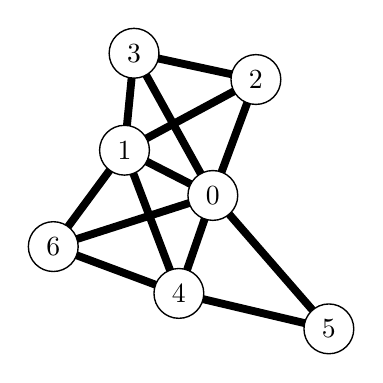
\begin{tikzpicture}[scale=0.70]
					\definecolor{cv0}{rgb}{0.0,0.0,0.0}
					\definecolor{cfv0}{rgb}{1.0,1.0,1.0}
					\definecolor{clv0}{rgb}{0.0,0.0,0.0}
					\definecolor{cv1}{rgb}{0.0,0.0,0.0}
					\definecolor{cfv1}{rgb}{1.0,1.0,1.0}
					\definecolor{clv1}{rgb}{0.0,0.0,0.0}
					\definecolor{cv2}{rgb}{0.0,0.0,0.0}
					\definecolor{cfv2}{rgb}{1.0,1.0,1.0}
					\definecolor{clv2}{rgb}{0.0,0.0,0.0}
					\definecolor{cv3}{rgb}{0.0,0.0,0.0}
					\definecolor{cfv3}{rgb}{1.0,1.0,1.0}
					\definecolor{clv3}{rgb}{0.0,0.0,0.0}
					\definecolor{cv4}{rgb}{0.0,0.0,0.0}
					\definecolor{cfv4}{rgb}{1.0,1.0,1.0}
					\definecolor{clv4}{rgb}{0.0,0.0,0.0}
					\definecolor{cv5}{rgb}{0.0,0.0,0.0}
					\definecolor{cfv5}{rgb}{1.0,1.0,1.0}
					\definecolor{clv5}{rgb}{0.0,0.0,0.0}
					\definecolor{cv6}{rgb}{0.0,0.0,0.0}
					\definecolor{cfv6}{rgb}{1.0,1.0,1.0}
					\definecolor{clv6}{rgb}{0.0,0.0,0.0}
					\definecolor{cv0v1}{rgb}{0.0,0.0,0.0}
					\definecolor{cv0v2}{rgb}{0.0,0.0,0.0}
					\definecolor{cv0v3}{rgb}{0.0,0.0,0.0}
					\definecolor{cv0v4}{rgb}{0.0,0.0,0.0}
					\definecolor{cv0v5}{rgb}{0.0,0.0,0.0}
					\definecolor{cv0v6}{rgb}{0.0,0.0,0.0}
					\definecolor{cv1v2}{rgb}{0.0,0.0,0.0}
					\definecolor{cv1v3}{rgb}{0.0,0.0,0.0}
					\definecolor{cv1v4}{rgb}{0.0,0.0,0.0}
					\definecolor{cv1v6}{rgb}{0.0,0.0,0.0}
					\definecolor{cv2v3}{rgb}{0.0,0.0,0.0}
					\definecolor{cv4v5}{rgb}{0.0,0.0,0.0}
					\definecolor{cv4v6}{rgb}{0.0,0.0,0.0}
					%
					\Vertex[style={minimum size=1.0cm,draw=cv0,fill=cfv0,text=clv0,shape=circle},LabelOut=false,L=\hbox{$0$},x=2.8949cm,y=2.4204cm]{v0}
					\Vertex[style={minimum size=1.0cm,draw=cv1,fill=cfv1,text=clv1,shape=circle},LabelOut=false,L=\hbox{$1$},x=1.2923cm,y=3.241cm]{v1}
					\Vertex[style={minimum size=1.0cm,draw=cv2,fill=cfv2,text=clv2,shape=circle},LabelOut=false,L=\hbox{$2$},x=3.6763cm,y=4.5237cm]{v2}
					\Vertex[style={minimum size=1.0cm,draw=cv3,fill=cfv3,text=clv3,shape=circle},LabelOut=false,L=\hbox{$3$},x=1.4656cm,y=5.0cm]{v3}
					\Vertex[style={minimum size=1.0cm,draw=cv4,fill=cfv4,text=clv4,shape=circle},LabelOut=false,L=\hbox{$4$},x=2.2789cm,y=0.643cm]{v4}
					\Vertex[style={minimum size=1.0cm,draw=cv5,fill=cfv5,text=clv5,shape=circle},LabelOut=false,L=\hbox{$5$},x=5.0cm,y=0.0cm]{v5}
					\Vertex[style={minimum size=1.0cm,draw=cv6,fill=cfv6,text=clv6,shape=circle},LabelOut=false,L=\hbox{$6$},x=0.0cm,y=1.4924cm]{v6}
					%
					\Edge[lw=0.1cm,style={color=cv0v1,},](v0)(v1)
					\Edge[lw=0.1cm,style={color=cv0v2,},](v0)(v2)
					\Edge[lw=0.1cm,style={color=cv0v3,},](v0)(v3)
					\Edge[lw=0.1cm,style={color=cv0v4,},](v0)(v4)
					\Edge[lw=0.1cm,style={color=cv0v5,},](v0)(v5)
					\Edge[lw=0.1cm,style={color=cv0v6,},](v0)(v6)
					\Edge[lw=0.1cm,style={color=cv1v2,},](v1)(v2)
					\Edge[lw=0.1cm,style={color=cv1v3,},](v1)(v3)
					\Edge[lw=0.1cm,style={color=cv1v4,},](v1)(v4)
					\Edge[lw=0.1cm,style={color=cv1v6,},](v1)(v6)
					\Edge[lw=0.1cm,style={color=cv2v3,},](v2)(v3)
					\Edge[lw=0.1cm,style={color=cv4v5,},](v4)(v5)
					\Edge[lw=0.1cm,style={color=cv4v6,},](v4)(v6)
					%
				\end{tikzpicture}
			\end{center}
		\caption{The graph $T^2$.}
	\end{subfigure}
		%\end{subfigure}
	\begin{subfigure}[s]{0.3\textwidth}
		\begin{center}
		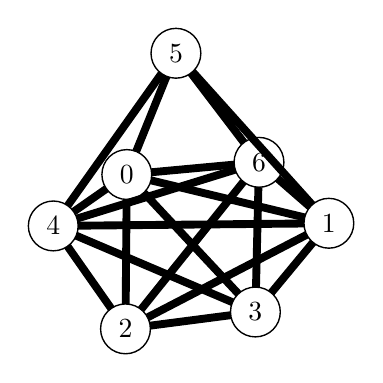
\begin{tikzpicture}[scale = 0.70]
			\definecolor{cv0}{rgb}{0.0,0.0,0.0}
			\definecolor{cfv0}{rgb}{1.0,1.0,1.0}
			\definecolor{clv0}{rgb}{0.0,0.0,0.0}
			\definecolor{cv1}{rgb}{0.0,0.0,0.0}
			\definecolor{cfv1}{rgb}{1.0,1.0,1.0}
			\definecolor{clv1}{rgb}{0.0,0.0,0.0}
			\definecolor{cv2}{rgb}{0.0,0.0,0.0}
			\definecolor{cfv2}{rgb}{1.0,1.0,1.0}
			\definecolor{clv2}{rgb}{0.0,0.0,0.0}
			\definecolor{cv3}{rgb}{0.0,0.0,0.0}
			\definecolor{cfv3}{rgb}{1.0,1.0,1.0}
			\definecolor{clv3}{rgb}{0.0,0.0,0.0}
			\definecolor{cv4}{rgb}{0.0,0.0,0.0}
			\definecolor{cfv4}{rgb}{1.0,1.0,1.0}
			\definecolor{clv4}{rgb}{0.0,0.0,0.0}
			\definecolor{cv5}{rgb}{0.0,0.0,0.0}
			\definecolor{cfv5}{rgb}{1.0,1.0,1.0}
			\definecolor{clv5}{rgb}{0.0,0.0,0.0}
			\definecolor{cv6}{rgb}{0.0,0.0,0.0}
			\definecolor{cfv6}{rgb}{1.0,1.0,1.0}
			\definecolor{clv6}{rgb}{0.0,0.0,0.0}
			\definecolor{cv0v1}{rgb}{0.0,0.0,0.0}
			\definecolor{cv0v2}{rgb}{0.0,0.0,0.0}
			\definecolor{cv0v3}{rgb}{0.0,0.0,0.0}
			\definecolor{cv0v4}{rgb}{0.0,0.0,0.0}
			\definecolor{cv0v5}{rgb}{0.0,0.0,0.0}
			\definecolor{cv0v6}{rgb}{0.0,0.0,0.0}
			\definecolor{cv1v2}{rgb}{0.0,0.0,0.0}
			\definecolor{cv1v3}{rgb}{0.0,0.0,0.0}
			\definecolor{cv1v4}{rgb}{0.0,0.0,0.0}
			\definecolor{cv1v5}{rgb}{0.0,0.0,0.0}
			\definecolor{cv1v6}{rgb}{0.0,0.0,0.0}
			\definecolor{cv2v3}{rgb}{0.0,0.0,0.0}
			\definecolor{cv2v4}{rgb}{0.0,0.0,0.0}
			\definecolor{cv2v6}{rgb}{0.0,0.0,0.0}
			\definecolor{cv3v4}{rgb}{0.0,0.0,0.0}
			\definecolor{cv3v6}{rgb}{0.0,0.0,0.0}
			\definecolor{cv4v5}{rgb}{0.0,0.0,0.0}
			\definecolor{cv4v6}{rgb}{0.0,0.0,0.0}
			\definecolor{cv5v6}{rgb}{0.0,0.0,0.0}
			%
			\Vertex[style={minimum size=1.0cm,draw=cv0,fill=cfv0,text=clv0,shape=circle},LabelOut=false,L=\hbox{$0$},x=1.3342cm,y=2.8cm]{v0}
			\Vertex[style={minimum size=1.0cm,draw=cv1,fill=cfv1,text=clv1,shape=circle},LabelOut=false,L=\hbox{$1$},x=5.0cm,y=1.9158cm]{v1}
			\Vertex[style={minimum size=1.0cm,draw=cv2,fill=cfv2,text=clv2,shape=circle},LabelOut=false,L=\hbox{$2$},x=1.3103cm,y=0.0cm]{v2}
			\Vertex[style={minimum size=1.0cm,draw=cv3,fill=cfv3,text=clv3,shape=circle},LabelOut=false,L=\hbox{$3$},x=3.667cm,y=0.3062cm]{v3}
			\Vertex[style={minimum size=1.0cm,draw=cv4,fill=cfv4,text=clv4,shape=circle},LabelOut=false,L=\hbox{$4$},x=0.0cm,y=1.8675cm]{v4}
			\Vertex[style={minimum size=1.0cm,draw=cv5,fill=cfv5,text=clv5,shape=circle},LabelOut=false,L=\hbox{$5$},x=2.2253cm,y=5.0cm]{v5}
			\Vertex[style={minimum size=1.0cm,draw=cv6,fill=cfv6,text=clv6,shape=circle},LabelOut=false,L=\hbox{$6$},x=3.7324cm,y=3.0213cm]{v6}
			%
			\Edge[lw=0.1cm,style={color=cv0v1,},](v0)(v1)
			\Edge[lw=0.1cm,style={color=cv0v2,},](v0)(v2)
			\Edge[lw=0.1cm,style={color=cv0v3,},](v0)(v3)
			\Edge[lw=0.1cm,style={color=cv0v4,},](v0)(v4)
			\Edge[lw=0.1cm,style={color=cv0v5,},](v0)(v5)
			\Edge[lw=0.1cm,style={color=cv0v6,},](v0)(v6)
			\Edge[lw=0.1cm,style={color=cv1v2,},](v1)(v2)
			\Edge[lw=0.1cm,style={color=cv1v3,},](v1)(v3)
			\Edge[lw=0.1cm,style={color=cv1v4,},](v1)(v4)
			\Edge[lw=0.1cm,style={color=cv1v5,},](v1)(v5)
			\Edge[lw=0.1cm,style={color=cv1v6,},](v1)(v6)
			\Edge[lw=0.1cm,style={color=cv2v3,},](v2)(v3)
			\Edge[lw=0.1cm,style={color=cv2v4,},](v2)(v4)
			\Edge[lw=0.1cm,style={color=cv2v6,},](v2)(v6)
			\Edge[lw=0.1cm,style={color=cv3v4,},](v3)(v4)
			\Edge[lw=0.1cm,style={color=cv3v6,},](v3)(v6)
			\Edge[lw=0.1cm,style={color=cv4v5,},](v4)(v5)
			\Edge[lw=0.1cm,style={color=cv4v6,},](v4)(v6)
			\Edge[lw=0.1cm,style={color=cv5v6,},](v5)(v6)
			%
		\end{tikzpicture}
	\end{center}
	\caption{The graph $T^3$.}
	\end{subfigure}
	\begin{subfigure}[s]{0.3\textwidth}
	\begin{center}
		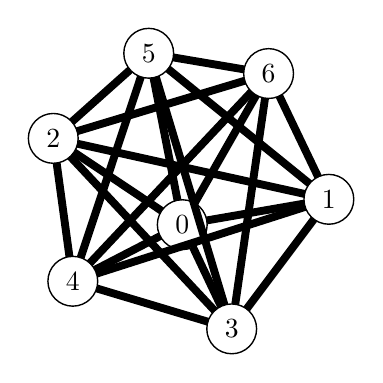
\begin{tikzpicture}[scale=0.70]
			\definecolor{cv0}{rgb}{0.0,0.0,0.0}
			\definecolor{cfv0}{rgb}{1.0,1.0,1.0}
			\definecolor{clv0}{rgb}{0.0,0.0,0.0}
			\definecolor{cv1}{rgb}{0.0,0.0,0.0}
			\definecolor{cfv1}{rgb}{1.0,1.0,1.0}
			\definecolor{clv1}{rgb}{0.0,0.0,0.0}
			\definecolor{cv2}{rgb}{0.0,0.0,0.0}
			\definecolor{cfv2}{rgb}{1.0,1.0,1.0}
			\definecolor{clv2}{rgb}{0.0,0.0,0.0}
			\definecolor{cv3}{rgb}{0.0,0.0,0.0}
			\definecolor{cfv3}{rgb}{1.0,1.0,1.0}
			\definecolor{clv3}{rgb}{0.0,0.0,0.0}
			\definecolor{cv4}{rgb}{0.0,0.0,0.0}
			\definecolor{cfv4}{rgb}{1.0,1.0,1.0}
			\definecolor{clv4}{rgb}{0.0,0.0,0.0}
			\definecolor{cv5}{rgb}{0.0,0.0,0.0}
			\definecolor{cfv5}{rgb}{1.0,1.0,1.0}
			\definecolor{clv5}{rgb}{0.0,0.0,0.0}
			\definecolor{cv6}{rgb}{0.0,0.0,0.0}
			\definecolor{cfv6}{rgb}{1.0,1.0,1.0}
			\definecolor{clv6}{rgb}{0.0,0.0,0.0}
			\definecolor{cv0v1}{rgb}{0.0,0.0,0.0}
			\definecolor{cv0v2}{rgb}{0.0,0.0,0.0}
			\definecolor{cv0v3}{rgb}{0.0,0.0,0.0}
			\definecolor{cv0v4}{rgb}{0.0,0.0,0.0}
			\definecolor{cv0v5}{rgb}{0.0,0.0,0.0}
			\definecolor{cv0v6}{rgb}{0.0,0.0,0.0}
			\definecolor{cv1v2}{rgb}{0.0,0.0,0.0}
			\definecolor{cv1v3}{rgb}{0.0,0.0,0.0}
			\definecolor{cv1v4}{rgb}{0.0,0.0,0.0}
			\definecolor{cv1v5}{rgb}{0.0,0.0,0.0}
			\definecolor{cv1v6}{rgb}{0.0,0.0,0.0}
			\definecolor{cv2v3}{rgb}{0.0,0.0,0.0}
			\definecolor{cv2v4}{rgb}{0.0,0.0,0.0}
			\definecolor{cv2v5}{rgb}{0.0,0.0,0.0}
			\definecolor{cv2v6}{rgb}{0.0,0.0,0.0}
			\definecolor{cv3v4}{rgb}{0.0,0.0,0.0}
			\definecolor{cv3v5}{rgb}{0.0,0.0,0.0}
			\definecolor{cv3v6}{rgb}{0.0,0.0,0.0}
			\definecolor{cv4v5}{rgb}{0.0,0.0,0.0}
			\definecolor{cv4v6}{rgb}{0.0,0.0,0.0}
			\definecolor{cv5v6}{rgb}{0.0,0.0,0.0}
			%
			\Vertex[style={minimum size=1.0cm,draw=cv0,fill=cfv0,text=clv0,shape=circle},LabelOut=false,L=\hbox{$0$},x=2.3403cm,y=1.8902cm]{v0}
			\Vertex[style={minimum size=1.0cm,draw=cv1,fill=cfv1,text=clv1,shape=circle},LabelOut=false,L=\hbox{$1$},x=5.0cm,y=2.3503cm]{v1}
			\Vertex[style={minimum size=1.0cm,draw=cv2,fill=cfv2,text=clv2,shape=circle},LabelOut=false,L=\hbox{$2$},x=0.0cm,y=3.4559cm]{v2}
			\Vertex[style={minimum size=1.0cm,draw=cv3,fill=cfv3,text=clv3,shape=circle},LabelOut=false,L=\hbox{$3$},x=3.2372cm,y=0.0cm]{v3}
			\Vertex[style={minimum size=1.0cm,draw=cv4,fill=cfv4,text=clv4,shape=circle},LabelOut=false,L=\hbox{$4$},x=0.3545cm,y=0.8637cm]{v4}
			\Vertex[style={minimum size=1.0cm,draw=cv5,fill=cfv5,text=clv5,shape=circle},LabelOut=false,L=\hbox{$5$},x=1.7316cm,y=5.0cm]{v5}
			\Vertex[style={minimum size=1.0cm,draw=cv6,fill=cfv6,text=clv6,shape=circle},LabelOut=false,L=\hbox{$6$},x=3.9064cm,y=4.6319cm]{v6}
			%
			\Edge[lw=0.1cm,style={color=cv0v1,},](v0)(v1)
			\Edge[lw=0.1cm,style={color=cv0v2,},](v0)(v2)
			\Edge[lw=0.1cm,style={color=cv0v3,},](v0)(v3)
			\Edge[lw=0.1cm,style={color=cv0v4,},](v0)(v4)
			\Edge[lw=0.1cm,style={color=cv0v5,},](v0)(v5)
			\Edge[lw=0.1cm,style={color=cv0v6,},](v0)(v6)
			\Edge[lw=0.1cm,style={color=cv1v2,},](v1)(v2)
			\Edge[lw=0.1cm,style={color=cv1v3,},](v1)(v3)
			\Edge[lw=0.1cm,style={color=cv1v4,},](v1)(v4)
			\Edge[lw=0.1cm,style={color=cv1v5,},](v1)(v5)
			\Edge[lw=0.1cm,style={color=cv1v6,},](v1)(v6)
			\Edge[lw=0.1cm,style={color=cv2v3,},](v2)(v3)
			\Edge[lw=0.1cm,style={color=cv2v4,},](v2)(v4)
			\Edge[lw=0.1cm,style={color=cv2v5,},](v2)(v5)
			\Edge[lw=0.1cm,style={color=cv2v6,},](v2)(v6)
			\Edge[lw=0.1cm,style={color=cv3v4,},](v3)(v4)
			\Edge[lw=0.1cm,style={color=cv3v5,},](v3)(v5)
			\Edge[lw=0.1cm,style={color=cv3v6,},](v3)(v6)
			\Edge[lw=0.1cm,style={color=cv4v5,},](v4)(v5)
			\Edge[lw=0.1cm,style={color=cv4v6,},](v4)(v6)
			\Edge[lw=0.1cm,style={color=cv5v6,},](v5)(v6)
			%
		\end{tikzpicture}
	\end{center}
	\caption{The graph $T^4$.}
	\end{subfigure}
	\end{figure}
\end{eg}
\newpage

When the triangle bases are nested (when can this be the case?), it is easy to partition the cycle space of $G^{\diam}$ into orthogonal subspaces, each with dimension equal the distance multiplicities.  In general, it is always possible to do this, however, if the triangle bases aren't nested, it seems less obvious how to partition into orthogonal subspaces corresponding to the distances.  We denote such a subspace for distance $k$ by $\mathcal{M}_k$.  In the above example, these subspaces are:
\begin{align*}
	\mathcal{M}_2 &= \subspan(\{160, 460, 450, 140, 130, 230, 120\})	\\
	\mathcal{M}_3 &= \subspan(\{260, 360, 560, 150, 240, 340\})	\\
	\mathcal{M}_4 &= \subspan(\{350, 250\}).
\end{align*}

I believe it's a coincidence that all triangles in this example contain $0$.  There are $k$-triangle bases that must contain disjoint triangles, specifically when $k$ is not near the diameter.

\section{Observations}
\begin{enumerate}
	\item The number of non-zero entries of $A(G)^k$ is equal to $|E(G^k)|$.  This seems like a good way to relate $A(G^k)$ with $A(G)$.  Note that this means that $m(k)$ is the difference of number of vertex pairs with walks of length $k$ and number of vertex pairs with walks of length $k-1$.
	\item The cycle space of $G$ is the null space of the $n \times {n \choose 2}$ vertex-edge incidence matrix of $G$.  Maybe we can use this to study $\mathcal{M}_k$ or $k$-triangle bases somehow.
	\item Since triangles are either disjoint, share 1 edge, or are equal, it seems like it ought to be a good idea to consider an triangle-edge incidence matrix for $G^k$ here too.
	\item There is a relationship between $\mathcal{C}(G^{\diam})$ and the distance matrix for $G$.  Let $T$ be a spanning tree of $G$.  Then colour all edges of $G$ with $1$, and then for each fundamental cycle of the form $T+uv$, where $uv \in E(G^{\diam})\setminus E(G)$, colour $uv$ with $d(u,v)$.  The result is a distance edge weighted complete graph, whose adjacency matrix is the distance matrix for $G$.
\end{enumerate}

\section{Questions}

\begin{enumerate}
	\item It could be interesting to explore questions that relate these cycle subspaces $\mathcal{T}(G^k)$ and $\mathcal{M}_k$ with graph structure.  For instance, suppose $T_1$ and $T_2$ have the same multiplicity of distance $k$.  When is it possible for them to have intersecting, or equal, triangle bases?
	\item Inversely, suppose $T_1$ and $T_2$ have the same $k$-triangle basis.  Then how do they relate in structure as trees?  Merely having the same multiplicity for distance $k$ doesn't necessarily imply (I don't think) that $T_1$ and $T_2$ can share a $k$-triangle basis.
	\item How exactly does distance $k$ show up in all vectors in $\mathcal{M}_k$?  I think each subgraph in $\mathcal{M}_k$ has a pair of vertices at distance $k$.  Also, I suppose any graph with all pairs at distance $k$ in $G$, must be in $\mathcal{M}_k$.  I think it might be the case that a graph $R$ is in $\mathcal{M}_k$ if and only if its max (non-infinity if disconnected) distance is equal to $k$ in $G$.
	\item Can we characterize the graphs corresponding to $\sum_{x \in \mathcal{M}_k} x$?
	\item Suppose we find a formula for $m(k)$ in terms of $A(G^k)$.  Can we find a way to express it in terms of $A(G)$?
	\item Anyway, I think there could be a variety of interesting questions to ask here!
\end{enumerate}

\iffalse
\section{Observations and Facts}

\subsection{Key Idea}

We know the distance multiplicities if we know the number of edges in the powers of the graph, which we can get from the dimension of its cycle space.  Since the span of all induced cycles equals the cycle space, when the graph powers are chordal, some subset of triangles in the graph power form a basis for the cycle space.  

\subsection{Related Matrices}

\begin{itemize}
	\item Incidence matrix for the graph $G^k$.  The null space of this matrix is the cycle space.  So, the dimension of the null space of this matrix is essentially the number of edges in $G^k$.
	\item Edge-Triangle inclusion matrix?
	\item Adjacency matrix of graph powers
	\item Number of edges in $G^k$ is equal to the number of non-zero entries of the $k$-th power of the adjacency matrix of $G$, $A_G^k$.  So, $m(k)$ is the difference of number of vertex pairs with walks of length $k$ and walks of length $k-1$.
\end{itemize}

\newpage
\section{Combinatorial and Algebraic Questions}
\begin{itemize}
	\item Since distance multiplicities of $G$ are differences in dimensions of cycles spaces of consecutive powers, $\dim\mathcal{C}(G^k) - \dim\mathcal{C}(G^{k-1})$, we can construct a triangle basis for the cycle space of $K_n$ that is partitioned into triangle bases for orthogonal subspaces, each with dimension equal to one of the distance multiplicities in $G$.  In this sense, we can associate a distance $2, 3, \ldots, \diam$ to each triangle in the basis of fundamental cycles for $G^{\diam}$.  Note that $G^{\diam} \sim K_n$, so such an association is actually equivalent to a distance colouring of the edges of $K_n$, which has weighted adjacency matrix equal to the distance matrix of $G$.  So, these triangle bases provide a way to link $A(G)$, $A(G^k)$, $B(G^k)$, and $D(G)$.  I think there are some pretty pictures here: First, we start with a $K_n$, and then we can colour triangles depending on which of the orthogonal ``distance" subspaces they are in.
	\item Make such a picture.
	\item Study the graphs in the span of the $k$-triangle basis.  The dimension of this space equals $m(k)$, and the triangles are fundamental triangles in $G^k$ that are not in $G^{k-1}$, that is, they involve an edge $uv$ such that $d(u,v) = k$.  Note that when $G$ is a tree, this triangle corresponds to the unique cycle in $T+uv$.
	\item Let $t_k$ be the number of triangles in $G^k$.  That is, $t_k := \tfrac{Tr(A^3(G^k))}{6}$.  Let $W_k$ be the $t_k \times {n \choose 2}$ inclusion matrix for $G^k$.  Note that no two distinct triangles can share $2$ edges.  Here, we Then if $\mathcal{T}_k$ is a $k$-triangle basis, then for each $v \in \mathcal{T}_k$, 
	$$(W_k - W_{k-1})v = \mathbb{1}_v(i) = \begin{cases}
		1, \text{if } v = W_i	\\
		0, \text{otherwise.}
	\end{cases}$$
\end{itemize}
\fi

\newpage

\section{Cycle Space Partition}

Let $\mathcal{M}_k$ be the subspace of $\mathcal{C}(G^{k})$ generated by all triangles containing a distance $k$ edge.  Equivalently, $\mathcal{M}_k$ is the set of characteristic vectors in $\mathbb{F}^{n \choose 2}$ of all eulerian subgraphs of $G^k$ that are not in $G^{k-1}$.  Observe that $\dim\mathcal{M}_k = m(k)$.  Below we prove a lemma that shows the existence of a basis for $\mathcal{M}_k$ involving triangles with exactly one distance $k$ edge.

\begin{lem}
	Let $T$ be a tree.  Then the set of triangles in $T^k$ involving exactly one distance $k$ edge are in bijection with the distance $k$ edges.
\end{lem}
\begin{proof}
	Contradict acyclicity.
\end{proof}

\begin{lem}
	There exists a basis for $\mathcal{M}_k$ in which all triangles have exactly one distance $k$ edge.
\end{lem}
\begin{proof}
	Show that the triangles must either be all dist. $k$ edges, or have a unique dist. $k$ edge.  Show that we may swap the ``all dist. $k$" triangles with unique dist. $k$ triangles outside the span of the basis.
\end{proof}

\begin{prop}
	It holds that $m(2) = t_2 - \#K_{1,3}$.
\end{prop}

\begin{thm}
	It holds that 
	$$m(k) = \begin{cases}
		t_k - t_{k-1}, &\text{if $k$ is odd;}	\\
		(t_k - \#K_{1,k/2}) - t_{k-1}, &\text{if $k$ is even.}
	\end{cases}$$
\end{thm}



Observe that we may order the edges of $G^k$ based on their distances, from low to high.  This means by Lemma [], the $m(k)$ triangles all have exactly one edge in the distance $k$ region of the characteristic vectors.
\end{document}